\documentclass{article}
% Packages used
% Packages
\usepackage{amssymb,amsmath,amsthm,bbm}
\usepackage{verbatim,float,url,dsfont}
\usepackage{graphicx,subfigure,psfrag}
\usepackage{algorithm,algorithmic}
\usepackage{mathtools,enumitem}
\usepackage{multirow}
\usepackage{ragged2e}
\usepackage{xr-hyper}
\usepackage{array}

\usepackage[colorlinks=true,citecolor=blue,urlcolor=blue,linkcolor=blue]{hyperref}
\usepackage[margin=1in]{geometry}
\usepackage[round]{natbib}

\usepackage[utf8]{inputenc} % allow utf-8 input
\usepackage[T1]{fontenc}    % use 8-bit T1 fonts
\usepackage{booktabs}       % professional-quality tables
\usepackage{nicefrac}         % compact symbols for 1/2, etc.
\usepackage{microtype}      % microtypography
\usepackage{pdflscape}

\ifdefined\TimesFont 
\usepackage{times} % use times font
\fi

\ifdefined\ParSkip 
\usepackage{parskip} % use par skip
\fi

% Place page number
\def\fillandplacepagenumber{%
 \par\pagestyle{empty}%
 \vbox to 0pt{\vss}\vfill
 \vbox to 0pt{\baselineskip0pt
   \hbox to\linewidth{\hss}%
   \baselineskip\footskip
   \hbox to\linewidth{%
     \hfil\thepage\hfil}\vss}}
     
% Theorems and such
\newtheorem{theorem}{Theorem}
\newtheorem{lemma}{Lemma}
\newtheorem{corollary}{Corollary}
\newtheorem{proposition}{Proposition}
\theoremstyle{definition}
\newtheorem{remark}{Remark}
\newtheorem{definition}{Definition}

% Assumption
\newtheorem*{assumption*}{\assumptionnumber}
\providecommand{\assumptionnumber}{}
\makeatletter
\newenvironment{assumption}[2]{
  \renewcommand{\assumptionnumber}{Assumption #1#2}
  \begin{assumption*}
  \protected@edef\@currentlabel{#1#2}}
{\end{assumption*}}
\makeatother

% Widebar
\makeatletter
\newcommand*\rel@kern[1]{\kern#1\dimexpr\macc@kerna}
\newcommand*\widebar[1]{%
  \begingroup
  \def\mathaccent##1##2{%
    \rel@kern{0.8}%
    \overline{\rel@kern{-0.8}\macc@nucleus\rel@kern{0.2}}%
    \rel@kern{-0.2}%
  }%
  \macc@depth\@ne
  \let\math@bgroup\@empty \let\math@egroup\macc@set@skewchar
  \mathsurround\z@ \frozen@everymath{\mathgroup\macc@group\relax}%
  \macc@set@skewchar\relax
  \let\mathaccentV\macc@nested@a
  \macc@nested@a\relax111{#1}%
  \endgroup
}
\makeatother

% Min and max 
\DeclareMathOperator*{\argmin}{argmin}
\DeclareMathOperator*{\argmax}{argmax}
\DeclareMathOperator*{\minimize}{minimize}
\DeclareMathOperator*{\maximize}{maximize}
\DeclareMathOperator*{\find}{find}
\DeclareMathOperator{\st}{subject\,\,to}

% Other operators
\DeclareMathOperator{\Cov}{Cov}
\DeclareMathOperator{\Var}{Var}
\DeclareMathOperator{\dm}{dim}
\DeclareMathOperator{\col}{col}
\DeclareMathOperator{\row}{row}
\DeclareMathOperator{\nul}{null}
\DeclareMathOperator{\rank}{rank}
\DeclareMathOperator{\nuli}{nullity}
\DeclareMathOperator{\spa}{span}
\DeclareMathOperator{\sign}{sign}
\DeclareMathOperator{\supp}{supp}
\DeclareMathOperator{\diag}{diag}
\DeclareMathOperator{\aff}{aff}
\DeclareMathOperator{\conv}{conv}
\DeclareMathOperator{\dom}{dom}
\DeclareMathOperator{\tr}{tr}
\DeclareMathOperator{\df}{df}

% Other shortcuts 
\def\R{\mathbb{R}}
\def\C{\mathbb{C}}
\def\E{\mathbb{E}}
\def\P{\mathbb{P}}
\def\T{\mathsf{T}}
\def\half{\frac{1}{2}}
\def\df{\mathrm{df}}
\def\hy{\hat{y}}
\def\hf{\hat{f}}
\def\hmu{\hat{\mu}}
\def\halpha{\hat{\alpha}}
\def\hbeta{\hat{\beta}}
\def\htheta{\hat{\theta}}
\def\indep{\perp\!\!\!\perp}
\def\th{^{\textnormal{th}}}

\def\cA{\mathcal{A}}
\def\cB{\mathcal{B}}
\def\cD{\mathcal{D}}
\def\cE{\mathcal{E}}
\def\cF{\mathcal{F}}
\def\cG{\mathcal{G}}
\def\cK{\mathcal{K}}
\def\cH{\mathcal{H}}
\def\cI{\mathcal{I}}
\def\cL{\mathcal{L}}
\def\cM{\mathcal{M}}
\def\cN{\mathcal{N}}
\def\cP{\mathcal{P}}
\def\cS{\mathcal{S}}
\def\cT{\mathcal{T}}
\def\cW{\mathcal{W}}
\def\cX{\mathcal{X}}
\def\cY{\mathcal{Y}}
\def\cZ{\mathcal{Z}}

 \def\given{\, \vert\, }

\def\TimesFont{} 
\graphicspath{{gfx/}}

\newcommand{\beginsupplement}{
  \setcounter{table}{1}  
  \renewcommand{\thetable}{S\arabic{table}} 
  \setcounter{figure}{1} 
  \renewcommand{\thefigure}{S\arabic{figure}}
  \setcounter{section}{0} 
  \renewcommand{\thesection}{S\arabic{section}}
}
\newcommand{\attn }[1]{\textcolor{red}{ATTN: #1}}

     
\begin{document}
\title{Retrospective estimation of latent COVID-19 infections over the pandemic in US states}
\author{Rachel Lobay, Maria Jahja, Ajitesh Srivastava, Ryan J. Tibshirani, Daniel J. McDonald}
\date{Version: \today}
\maketitle

\begin{abstract}
The true timing and magnitude of infections from the COVID-19 pandemic are of
interest to both the public and public health, but these are challenging to pin
down for a variety of data-driven and methodological reasons. Nonetheless, 
accurate estimates
of all latent infections can improve our understanding of the true size and
scope of the pandemic and provide an indication of disease patterns and burden
over time. In this work, we estimate the true daily incident infections for each
US state by deconvolving reported COVID-19 cases using estimated
infection-onset-to-case-report distributions followed by a serology-based
procedure to adjust for the unreported infections. We find clear
variability in the timing and magnitude in the resulting estimates, indicating a
differential impact of the pandemic across states and revealing a disease burden
that appears earlier and more extensively than indicated by cases alone. Our
findings help to better understand the impact of the pandemic in the US.
\end{abstract}

\section{Introduction}

Reported COVID-19 cases are a staple in tracking the pandemic at varying
geographic resolutions such as national, state and county levels
\citep{dong2020interactive, nyt2020corona, wp2020tracking}. Yet, for every case
that is eventually reported to public health, several infections are likely to
be missed. To see why, it is important to understand who's cases are being reported and,
in particular, what differentiates them from the unreported cases. Refer to
\autoref{fig:chain_events_onset_report} for an illustration of the path of a
symptomatic infection that is eventually reported to public health. 

Using this figure, we can discern a number of sources of bias in the reporting
pipeline. For instance, diagnostic testing mainly targets symptomatic
individuals; thus, infected individuals exhibiting little to no symptoms are
likely to be missed \citep{cdc2022estimated}. In addition, testing practices,
availability, and uptake vary across space and time \citep{pitzer2021impact,
ecdc2020strategies, hitchings2021usefulness}. Finally, cases provide a belated
view of the pandemic's progression because they are subject to delays due to the
viral incubation period, the speed and severity of symptom onset, laboratory
confirmation and test turnaround times, and submission to public health
\citep{pellis2021challenges, wash2020dash}. For these reasons, reported cases
are lagging indicators of the course of the pandemic. Furthermore, they do not
represent the actual number of new infections that occur on a given day, as
indicated by exposure to the pathogen. Ascertaining infection onset is difficult
because there was no large-scale surveillance effort in the United States that
reliably tracked symptom onset, let alone infection onset.

\begin{figure}[!tb]
\centering
    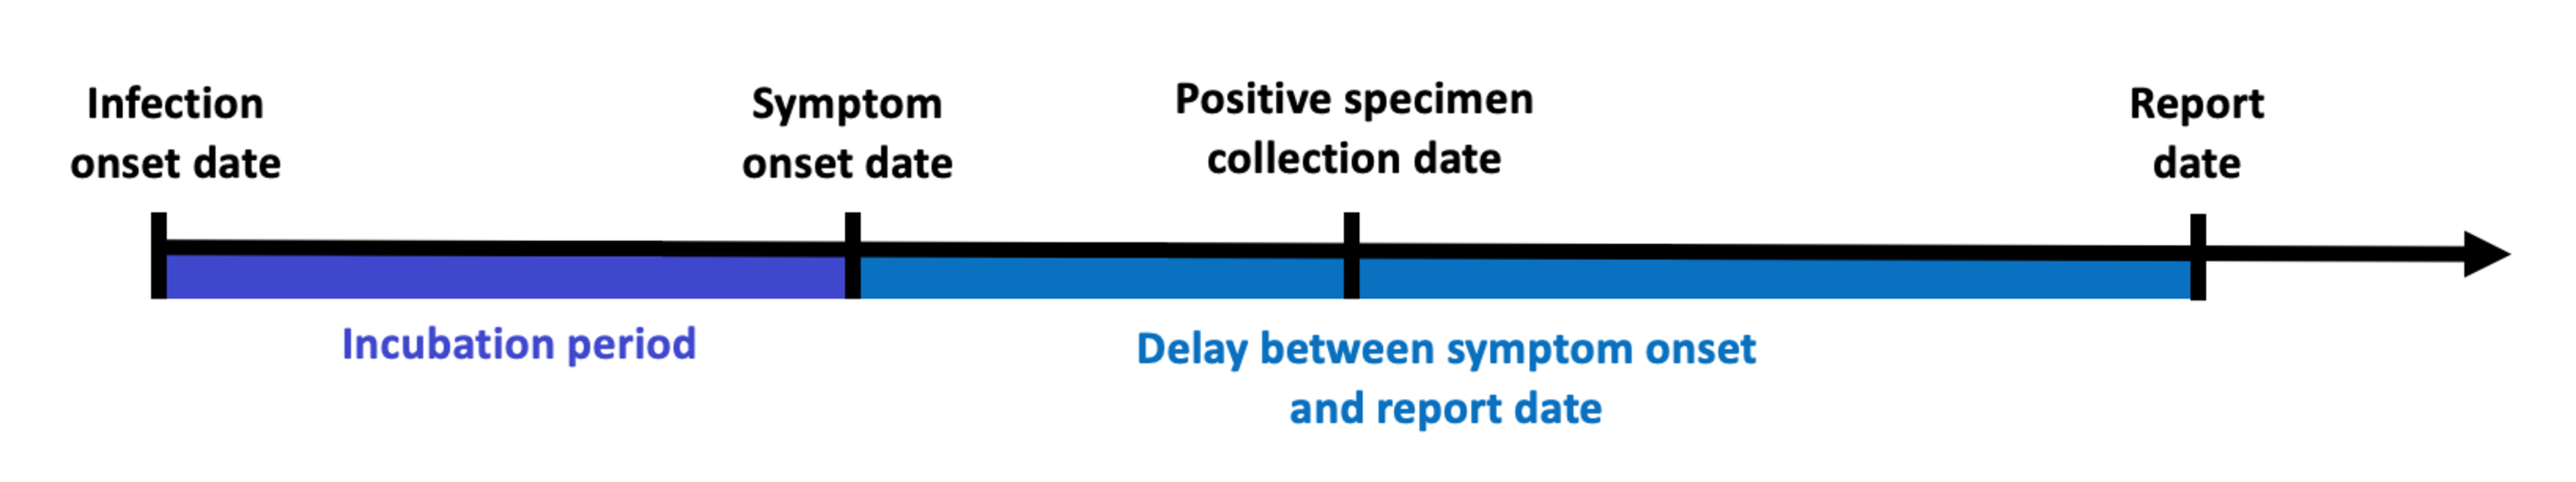
\includegraphics[width=.99\textwidth]{Chain_of_events_onset_report.pdf} 
    \caption{Idealized chain of events from infection onset to case report date 
    for a symptomatic infection that is eventually reported to public health.}
    \label{fig:chain_events_onset_report}
\end{figure}

% Importantly, all of these issues that are present in local health authority
% data are also present in the gold standard for case data from the JHU CSSE
% \citep{dong2020interactive, guidotti2022worldwide} because JHU scrapes case
% data from the local health authority dashboards \citep{jahja2022real}.
% Furthermore, the cases shown on the JHU CSSE Coronavirus Resource Center
% \citep{jhucsse2020covid} are those that have been disseminated to the public
% on a given day. 
% Our approach to estimate latent infections takes case data and estimates the 
% following...

Explaining the course of the pandemic and investigating the effects of
interventions, the burden facing various subgroups, and drawing insights for
future pandemics is challenging because the true spatial and temporal behaviour
is unknown. So while reported cases provide some understanding of the disease
burden in a population, it is incomplete, delayed, and understates the true size
of the pandemic. Regardless of these difficulties, it is important to the public
and public health to perform a pandemic post-mortem and try to better estimate the
true extent of its effect---to attempt to capture the true size and impact of
the pandemic as much as we can. Estimates of daily incident infections are one
such way to measure this and can guide public and professional understanding of
the pandemic burden over space and time.

In this work, we attempt to provide a statistically justified reconstruction of daily
incident infections for each US state from June 1, 2020 to Dec. 5, 2021. To our knowledge,
no other modelling approach has been used to reconstruct the infection time series for
each state over as large of a time interval. We achieve this by first breaking the task of 
estimating infection onset from report date into the more manageable parts of estimating the time 
from infection to symptom onset and the time from symptom onset to report date (as depicted in
\autoref{fig:chain_events_onset_report}). Using statewise data, we are able to construct 
state-time-specific incubation period and symptom-onset-to-case report delay distributions. 
We then use these estimated incubation period distributions in conjunction with their 
delay distributions to deconvolve daily reported COVID-19 cases to infection onset.
The resulting infection estimates are adjusted to
account for the unreported infections by using seroprevalence data in a novel leaky 
immunity model that is defined by its ability to account for the waning of detectable immunity.  
We examine some features of the adjusted estimates and the implications of
using them rather than reported cases. Comparing the correlations between adjusted
infections and state-level hospitalization data reveals much more believable delay
relationships than with reported cases. Relatedly, we demonstrate how to use our infection
estimates to compute time-varying infection-hospitalization ratios (IHRs) for each state,
and find \attn {...}. While these analyses provide a glimpse into the utility of our
infection estimates, we believe that there is much more to be explored, and we hope that
our work will prove an important benchmark for others to undertake retrospective analyses.

\section{Results}
%% Reminder to self - Consider to free y-axis on figures
%state_nia_est_faceted.pdf and state_niauc_est_faceted.pdf

% May decide to include figure for inverse reporting ratios in the appendix!
\begin{figure}[!tb]
\centering
    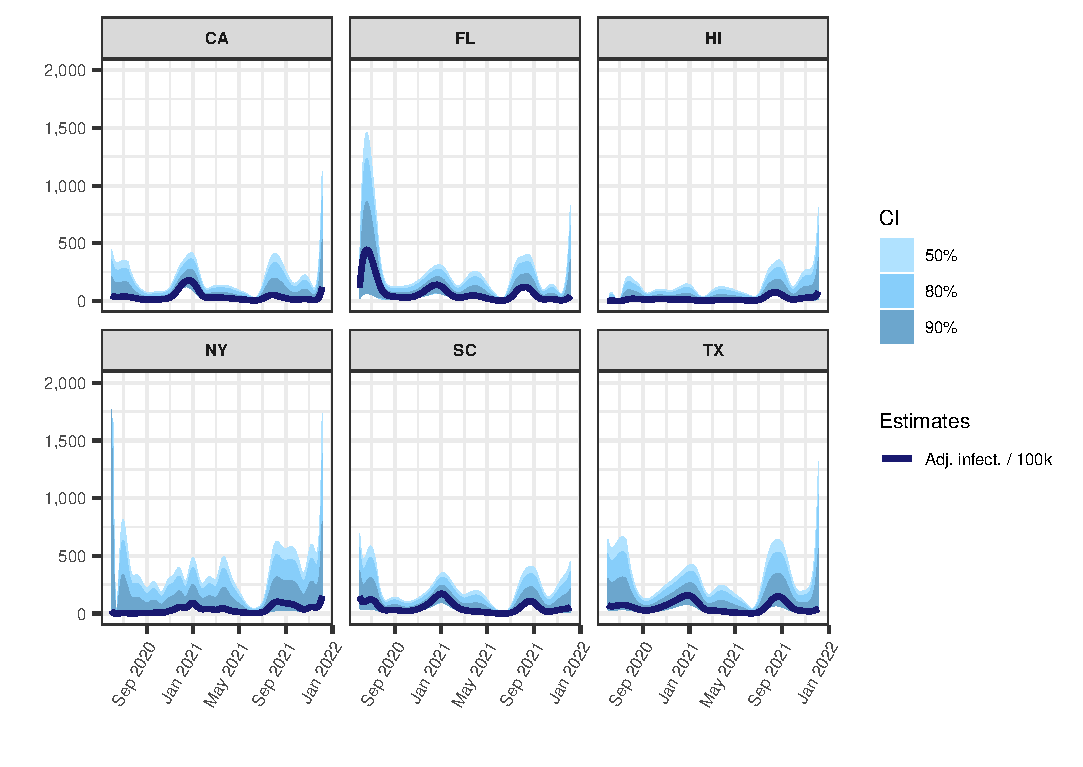
\includegraphics[width=.99\textwidth]{state_nia_est_faceted.pdf} 
    % Note extend this to all states (not just the sample of states)... So this
    % figure is currently more a preview
    \caption{Estimates of the number of daily new (adjusted) infections per 
    $100,000$ for each US state from June 1, 2020 to Dec. 5, 2021 (dark blue 
    line). The shaded regions depict the 50, 80, and 90\% confidence intervals.}
    \label{fig:state_nia_est_faceted}
\end{figure}

This work estimates incident infections for each US state over June 1,
2020 to December 5, 2021 and better illustrates the disease burden and viral
transmission dynamics at the state level across time. After converting the number
of infections to rates (infections per $100,000$ population), we look at
patterns in infections across the states and postulate what may be contributing
to these trends based on defining characteristics such as population density and 
composition and geographical contiguity. Finally, we perform a
brief comparison between infection and case estimates within each state and see
to what extent that surges in infections are apparent in both cases and infections
and instances where surges are only apparent from infections.

\subsection{Disease burden and viral transmission}
By reconstructing the time series of COVID-19 infections per $100,000$
population for each US state from June 1, 2020 to December 5, 2021, we observe
rates of infections that vary in intensity and disease burden across space and
time (\autoref{fig:state_nia_est_faceted} and \autoref{fig:chloro_inf_rates}).
The largest observed outbreak is over \rule{1cm}{0.15mm} in \rule{1cm}{0.15mm}
and \rule{1cm}{0.15mm}, suggesting a similar spread of the virus in states that
are in close geographic proximity. During this time, the state that has the
highest rate of infections per $100,000$ is \rule{1cm}{0.15mm} ($90\%$ CI
$[\rule{1cm}{0.15mm}]$) on \rule{1cm}{0.15mm}. Out of all infections in the
United States on that day, this comprises \rule{1cm}{0.15mm}\% ($90\%$ CI
$[\rule{1cm}{0.15mm}]$) of them. For these and most other states, smaller surges
can be observed in the fall of \rule{1cm}{0.15mm}, winter of \rule{1cm}{0.15mm},
and spring of \rule{1cm}{0.15mm}. Similar patterns in the major surges of
infections are observed in nearly all states, though to varying degrees. In
general, greater similarities in the strength and magnitude of outbreaks are
observed in the clusters of states that border each other and in those that have
similar population profiles in terms of age and other major medical risk factors
(such as obesity or chronic lung conditions). It is also notable that states
with high population density such as New Jersey, New York, and Rhode Island are
routinely subject to surges that are of greater in intensity and duration than
states with lower population density such as Alaska, Montana, and Wyoming.
% #%% Maybe this last sentence doesn't turn out to be true?

\begin{figure}[!tb]
\centering
    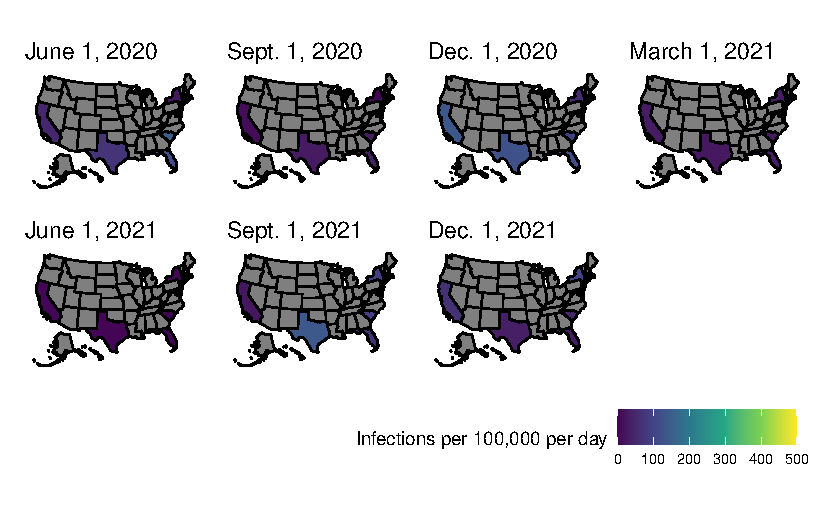
\includegraphics[width=.99\textwidth]{chloro_inf_rates.pdf}
    \caption{Chloropleth maps of the state-level estimates of the number of 
    daily new (adjusted) infections per $100,000$ population for various times 
    over June 1, 2020 to Dec. 5, 2021. These maps are generated from the \texttt{usmap} 
    package in R \citep{lorenzo2023usmap}.} 
    \label{fig:chloro_inf_rates}
\end{figure}

The period of lowest viral transmission is observed over the summer of \rule{1cm}{0.15mm},
where \rule{1cm}{0.15mm} achieves the lowest rate of infections on \rule{1cm}{0.15mm} (and
maintains a rate under \rule{1cm}{0.15mm} for a span of \rule{1cm}{0.15mm} days).
\rule{1cm}{0.15mm} states (\rule{1cm}{0.15mm}, \rule{1cm}{0.15mm} and \rule{1cm}{0.15mm})
meets the Centers for Disease Control and Prevention (CDC)’s definition of having a low
level of coronavirus transmission for that time of at most \rule{1cm}{0.15mm} new cases
per $100,000$ per week. As expected, the states that consistently achieve the lowest rates
of infections are those with the lowest population density (Montana and Wyoming) and/or
are geographically removed from the contiguous United States (Alaska and Hawaii). % Add
% reference for the CDC's definition of having a low level of coronavirus when know the
% specific time this applies to

From a brief inspection of the geo-contiguous states, we can observe similar patterns in
surges and periods of waning over time, suggesting that states who share similarities in
climate and topography performed similarly to each other. More precisely, we can observe
neighboring states such as New York and New Jersey or North Dakota and South Dakota that
present waves that mirror each other in amplitude and timing.

\subsection{Sensitivity analysis}
The infection estimates exhibit modest changes under different assumptions about the
variant-specific incubation periods, the construction of the delay distribution (the
window size for the considered onset dates), the fraction of new infections over time, and
the population estimates (see Supplementary Materials Section X). 
% \attn {Add a sentence or two about what is meant by modest changes... Did any of these result in noticeably higher or lower (biased) estimates of infections? To what extent (ie. an additional X infections)? For what states? Ablation stuff should also probably go here/near to this section.}
% Do these sensitivity analyses + update this link accordingly.

\subsection{Impact of analyzing infections rather than cases}
Naturally, outbreaks in infections precipitate those in cases and are reliably larger in
magnitude (\autoref{fig:state_niauc_est_faceted}). Hence, our infection estimates indicate
that the pandemic had a differential impact across states earlier and at a larger scale
than is suggested by cases. For many states in July 2020 and September 2021, there are
clear outbreaks in infections that are difficult to detect from cases alone, suggesting
that these are mainly comprised of unreported infections. Early on in the pandemic, such
discrepancies may be largely attributable to failures in the reporting pipeline, while
later on in the pandemic, they more likely due to the rise in asymptomatic infections
across variants \citep{oph2022covid, garrett2022high}.
\attn {We need some statements! The results can't just say, "we note
differences". What differences? What are the implications?}
Based on our infection estimates, we found that the total cases account for
\rule{1cm}{0.15mm}\% of the reported infections from June 1, 2020 to December 5, 2021.
% This last sentence may be making too much of a statement.

\begin{figure}[!tb]
\centering
    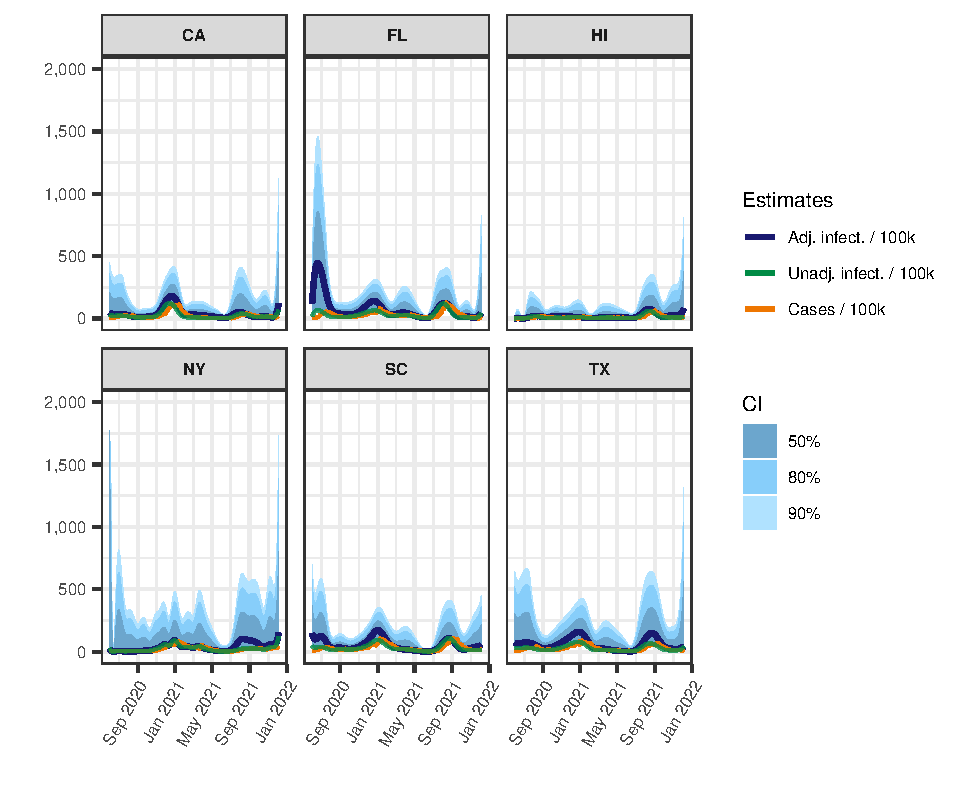
\includegraphics[width=.99\textwidth]{state_niauc_est_faceted.pdf} % Note extend this to all states (not just the sample of states)... So this figure is currently more a preview
    \caption{Estimates of the number of daily new (adjusted) infections per
     $100,000$ population for each US state from June 1, 2020 to Dec. 5, 2021
      (dark blue line). The shaded regions depict the 50, 80, and 90\% confidence 
      intervals for those adjusted estimates, while the teal line represents the 
      number of new daily new unadjusted infections per $100,000$, and the dotted 
      orange line represents the 7-day average of the new cases per $100,000$ as 
      of the same date.}
    \label{fig:state_niauc_est_faceted}
\end{figure}

We perform a lagged correlation analysis where we systematically investigate the
rank-based (ie. Spearman's) correlation between our infection and confirmed
hospitalization rates per $100,000$ population over a broad range of lag values
(\autoref{fig:infect_case_hosp_lag_corr}). Examining the correlation between infections and
hospitalizations shows that the maximum average correlation across states of $0.82$ is 
observed at a lag of $13$ days. In contrast, we find that the greatest average
rank-based correlations for cases with confirmed hospitalizations is achieved at a lag of
$0$. That is, we find that case report rates are nearly contemporaneous to
hospitalizations, while infection estimates clearly precede them. As a counterpart to our
lagged correlation analysis, we compute the time-varying IHRs for each state using the
optimal lag for infection and hospitalization rates (\autoref{fig:IHR_7dav}). 

\begin{figure}[!tb]
\centering
    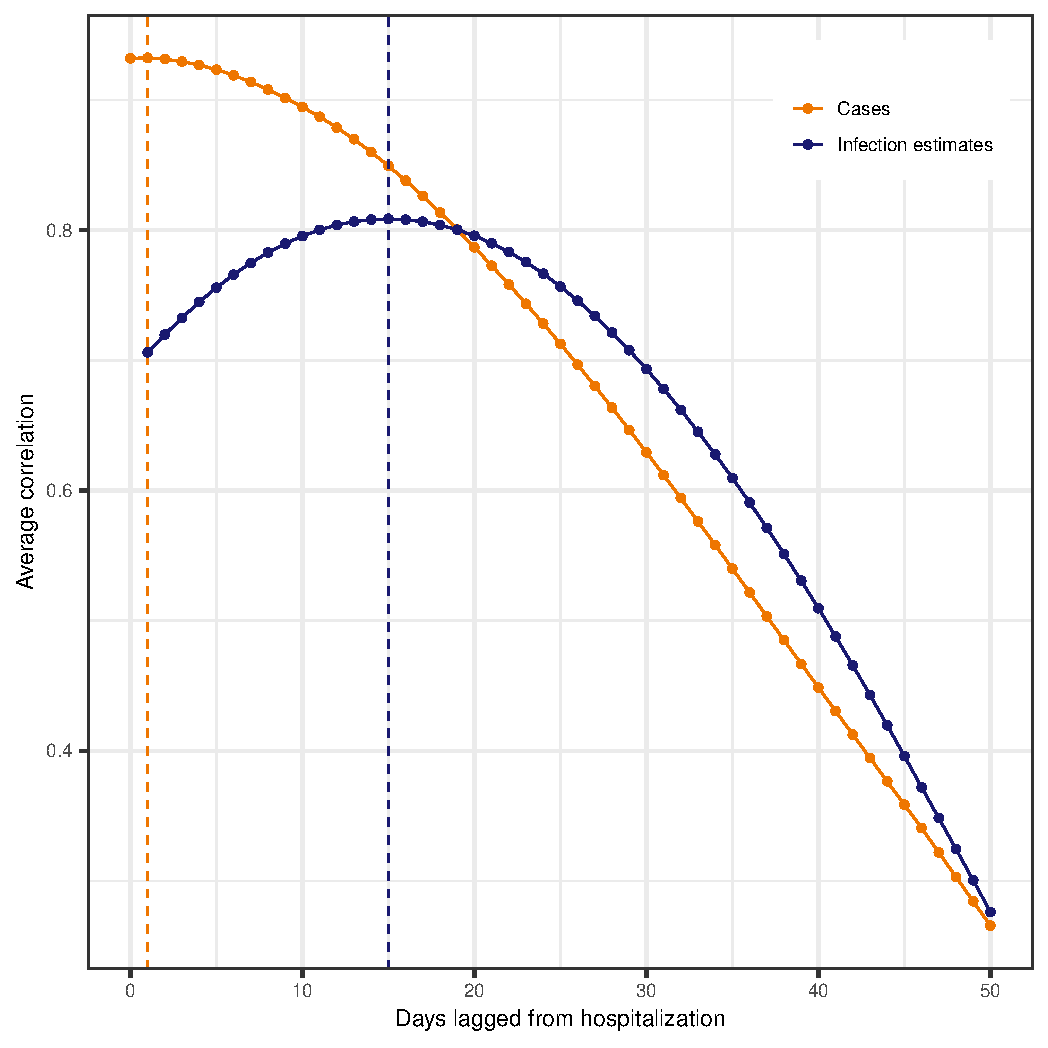
\includegraphics[width=.80\textwidth, height=.44\textheight]{infect_case_hosp_lag_corr.pdf} 
    \caption{Average rank-based correlation across US states between the infection and 
    hospitalization rates per $100,000$ (blue curve) as well as between case and 
    hospitalization rates per $100,000$ (orange curve) for a broad range of non-negative
     lag values. Note that infections, cases, and hospitalization counts are subject 
     to a center-aligned 7-day average to remove spurious day of the week effects. 
     The dashed lines indicate the lags for which the highest average correlation is attained.}
    \label{fig:infect_case_hosp_lag_corr}
\end{figure}

The IHRs that are obtained using this lag are generally small (in most cases less than
$0.1$ hospitalizations per infections and they exhibit similar geospatial and temporal trends 
as are noted for infections. Namely, states that are close in proximity (such as North Carolina 
and South Carolina) exhibit similar patterns in the IHRs over time. In addition, there are similar
spikes observed across many states at particular instances in time. For example, many
states such as Florida, Texas, and South Carolina exhibit a striking spike in
hospitalizations in mid-2021, which coincides with the rapid takeover of the Delta variant
during that time \citep{hodcroft2021covariants}. This finding aligns with previous studies
that found an increased risk in hospitalizations with Delta in comparison to other
variants \citep{twohig2022hospital, nyberg2022comparative}. Additionally, states that have
higher proportions of vulnerable populations such as the well-known retirement states of
Florida and Arizona are routinely subject to higher IHRs than other states. There may be
similar implications for states with a higher prevalence of medical risk factors such as
obesity or chronic lung diseases that are known to increase the risk of severe illness or
hospitalization from COVID-19 \citep{phc2020people, cdc2020people}. Overall the IHRs
presented similar geospatial and temporal trends as are observed for infections, but they
are generally less prominent and more constant across states and time. % More analysis
% later after decide on which IHRs (cumulative vs noncumualtive) to use. Can look into North
% vs South divide, which states had the consistently lowest IHRs, etc.

\begin{figure}[!tb]
\centering
    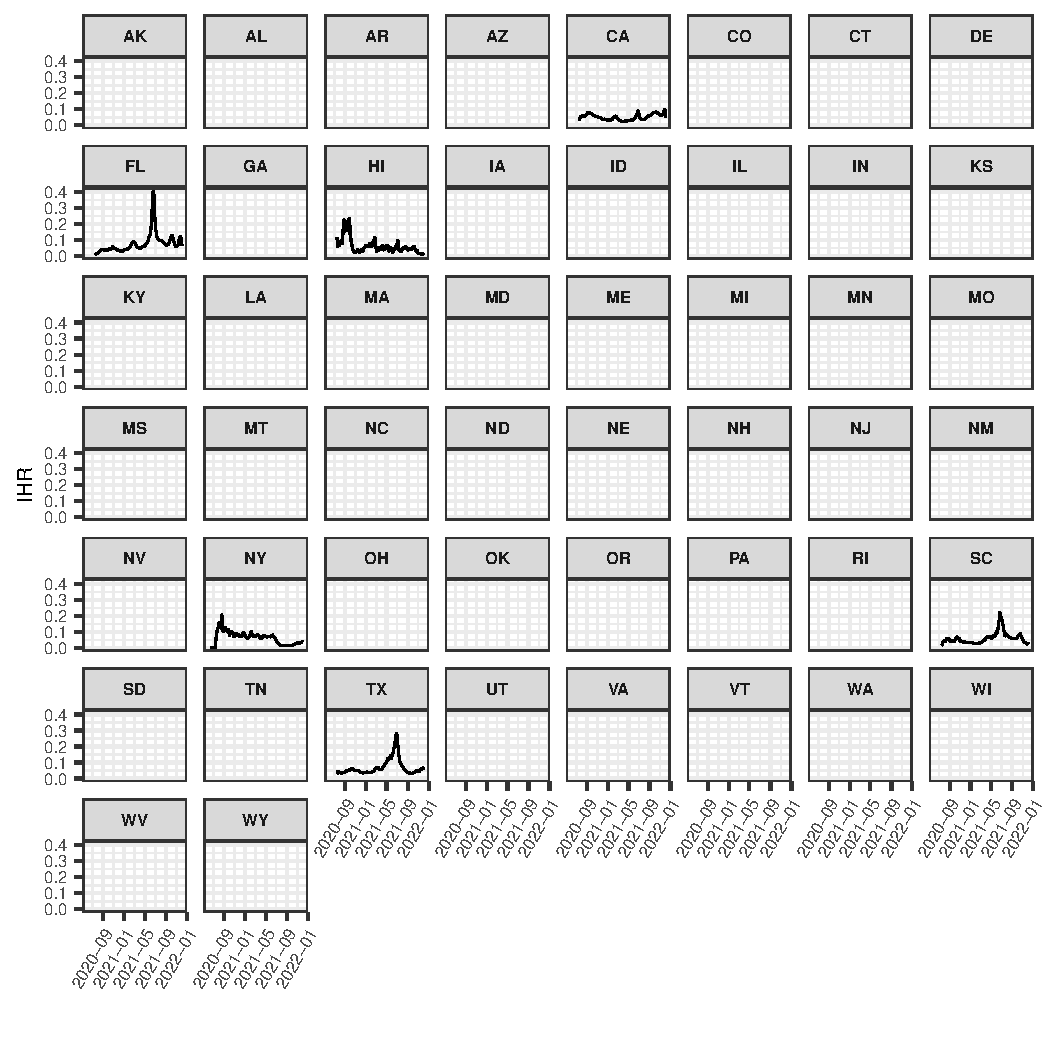
\includegraphics[width=.99\textwidth]{IHR_7dav.pdf} 
    \caption{Time-varying IHR estimates for each state from June 1, 2020 to Dec. 5, 2021 
    that are obtained using the optimal lag from the systematic lag analysis. 
    Note that the infection and hospitalization counts are subject to a 
    center-aligned 7-day average to remove spurious day of the week effects. 
    Also note that the different starting points across states are due to the 
    availability of the hospitalization data.}
    \label{fig:IHR_7dav}
\end{figure}

\section{Discussion}

We obtained retrospective estimates of daily incident infections for each US
state for June 1, 2020 to Dec. 5, 2021, which we will now discuss in more depth
and with respect to others' findings. The clear variability in the timing and
magnitude of our estimates indicate that the intensity and disease burden are
heterogenous across states. And yet, there are similar epidemic patterns such as
surges and periods of waning observed in clusters of neighboring states. In
addition, we observe that states of higher population density tended to suffer
from longer and more intense surges than states with lower population density,
which is supported by findings from both US and international studies
\citep{carozzi2022urban, iderus2022correlation, wong2020spreading}.
\citet{carozzi2022urban} suggests that the geographic connectivity and social
connectedness of denser areas can affect the timing of outbreaks, but they also
find that by the end of 2020 density had little to no impact on time-adjusted
COVID-19 cases. In simple terms, although dense locations are struck first, they
are not necessarily hit the hardest. However, further investigation beyond the
first year of the pandemic is warranted. As well, this study only looks relation
between density and cases, not infections (this same limitation applies to
\citet{jalal2021prominent}). The relationship between density and infections has
remained relatively unexplored and so a more detailed study of it is
warranted.
% Maybe the longer and more intense surges thing doesn't turn out to be true...
% It may be more that states with older populations and with a greater
% prevalence of chronic health conditions that areas major risk factors exhbit
% longer and more intense surges

Our infection estimates suggest that the pandemic has an impact
in states earlier and at a larger scale than is indicated by cases. Since
case reporting is not consistent across time and states, case counts
underestimate the true number of infections and, hence, the impact of the
pandemic \citep{cdc2022estimated, simon2022inconsistent}. For example, some
states report the number of individuals tested rather than the numbers of tests
performed \citep{schechtman2020counting, chitwood2021reconstructing}.

We observe outbreaks in infections that are virtually undetectable from cases
alone. \attn {examples} This suggests that cases provide an incomplete picture 
of the pandemic, especially with respect to outbreaks that are largely driven by 
unreported infections. Furthermore, since case report dates follow symptom and infection
onset, cases are a fundamentally flawed indicator of disease burden because they
have a built-in temporal bias. This is in addition to other biases from
differences in reporting across states (such as temporary bottlenecks due
influxes of data or more persistent processing issues that increase the average
time from case detection to report \citep{wash2020dash, dunkel2020covid19}. So
while reported cases provide an indication of the trajectory of the pandemic, it
is a delayed and incomplete version. Estimating the new number of infections by
symptom or infection onset date would more closely align with the definition of
incidence as we know it \citep{jahja2022real}.

From the correlation analysis between daily infection estimates and
hospitalizations, a lag of $13$ days gives the maximum average correlation
across states. This is commensurate with the early estimate of the average time
from infection to hospitalization of $9.7$ days ($95\%$ CI: $[5.4, 17.0]$) for
cases reported in January, 2020 in Wuhan, China as well as with estimates from
across the pandemic in the UK that ranged from an average of $8.0$ to $9.7$
days, more precisely, $8.0$ days ($95\%$ interval: $[2.7, 18.5]$) for the first
wave to $9.7$ days ($95\%$ interval: $[4.1, 19.6]$) for the second wave,
\citep{ward2021understanding}. However, we should note the first study is based
on a small sample size for outbreak cases reported well before our study start
date. As well, both sets of estimates depend upon the healthcare system and the
population structure, amongst other things \citep{ward2021understanding}.
Nevertheless, their relative agreement with our estimate of $13$ days for the US
states lends some credence to of our results. 

Although we computed IHRs for all states, the IHR is also likely to vary within
states and depend on additional variables such as age and the presence of major
comorbidities \citep{russell2023comorbidities}. Therefore, it would be
beneficial to account for such variables in the IHR calculations by, for
example, stratifying infections and hospitalizations by age to produce
age-specific estimates of the IHRs for each state (similar to
\citealt{fox2023disproportionate} though with the additional element of being
time-varying). We strongly believe this would be a worthwhile direction to
pursue in future work should the necessary information be available. 

The remainder of our discussion consists of an in-depth look into the advantages and
limitations of our approach and of other comparable approaches, followed by a
high level summary of our work and its major contributions. 

Our approach offers a number of advantages. The development 
of a way of modelling immunity and space-time-specific reporting ratios based on 
seroprevalence data is a major contribution. 
To the best of our knowledge, no other modelling approach has been used to 
reconstruct the infection time series
for every state over as much of the COVID-19 pandemic as in this study.
Furthermore, we aim to incorporate as much state-specific information as
possible when deriving our estimates. For instance, using variant circulation
and line list data, we are able to construct incubation and delay distributions
that were unique for each state. By using time-varying and state-specific
seroprevalence data, we are able to allow the reporting ratio to vary over both
time and state, which is an advantage over such ratios that are non-time varying
but state-specific and those that are time-varying but the same for all states
\citep{unwin2020state, uga2020covid19}. 
Existing approaches that use the delay distribution to generate infection
estimates often only construct one delay distribution that is used for all
states \citep{chitwood2021reconstructing, jahja2022real}. That is, they operate
under the assumption of geographic invariance, where it is assumed that all
states have the same patterns of delay from infection onset to case report,
which is unlikely to be true due to differences in reporting pipelines, pandemic
response, and variants in circulation, amongst other things. 

Another major limitation is that these models do not to account for
reinfections. Now, it may be contended that reinfections did not account for a
substantial fraction of the infections until later in the pandemic, so they were
not absolutely necessary to include in the earlier stages of the pandemic.
Still, at no stage did infection with the COVID-19 virus confer lifelong
immunity. Rather immunity is transient and wanes over time. And we believe it is
important to account for such defining characteristics of the virus when
tracking infections over time. Therefore, we account for reinfections and waning
of detectable immunity in our custom leaky immunity model. However, we 
acknowledge that the extent to which each of these are accounted for could be
improved upon in future work. 

Since the waning of detectable immunity is likely to be variant-dependent
\citep{pooley2023durability}, it follows that the leaky parameter may be better
posed as a mixture of parameters for different variants with weights determined
by the proportion of the variants circulating at the time in the state. Related
to this is the issue of how newer variants may escape detection
\citep{nih2022assessing, fda2023sars}. While in a retrospective analysis where
finalized data is used this is less likely to be an issue, this could very well
pose a problem for real-time estimates of infections.

As for reinfections, it would be ideal to have confirmed rates of reinfections
over time for each US state. However, we are unable to find such data available
over the entire time period considered for even one state. So we have turned to
suspected reinfection data over time for Clark County, USA, as that surveillance
is amongst the most detailed that we have found for the United States.
Nevertheless, using such localized data raises questions of representativeness
and the applicability of such estimates to Nevada and all other states.
Furthermore, this data has no information available beyond suspected third
infections, which imposes an irremediable bias. However, based on the third
infection data available there, we expect that the probability of being
reinfected more than three times is likely very low for time frame considered
and so the omission of these would impact our infection estimates to a small
extent. 

The vast majority of issues we encountered when trying to reconstruct the
infection time series for each state are due to an absence or a lack of data.
Such is the primary issue we had with the restricted line list. In comparison to
the number of JHU cases (which we are treating as a gold standard) for the same
release date, we noted there are about $10$ million cases that are unaccounted
for in the CDC line list. Moreover, the missingness does not appear to be random
and uniformly distributed across states, rather it is unequally distributed,
suggesting that the dataset may be biased. However, more information on the
cases that are missing versus present would be required to determine the extent
the missing cases led to a nonrepresentative, and therefore, biased sample, and
could be a topic of further study.

Seroprevalence data also runs the risk of being nonrepresentative of the
intended population \citep{bajema2021estimated}. For example, in the blood donor
dataset some states have region specific-estimates, which clearly do not stand
for the entire state. Another source of systematic variation is in the
characteristics of the individuals who opt for blood tests versus those who do
not. For instance, there may be a healthy user bias, in which a number of those
who opt for blood tests are generally more inclined to partake in proactive
healthy behaviors (such as checking on basic health markers by taking an annual
blood test) than those who do not \citep{parsley2018blood}. Alternatively, a
number of individuals may be recommended for blood tests by their doctors due to
signs of ill-health (ex. vitamin or mineral deficiencies or underlying medical
conditions). The extent that each such bias persists depends on the purpose of
the blood test and whether it was used as a proactive or reactive medical tool.
Since such information is unavailable to us, all we can conclude is that
participant-driven sources of bias impact the seroprevalence samples to an
undetermined extent. There are additional concerns about the performance of
antibody testing for individuals with mild or asymptomatic disease as well as
the loss of immunity over time \citep{kaku2021performance, seow2020longitudinal,
ibarrondo2020rapid}.

In this work, we do not attempt to directly address infection underascertainment
due to the increase in asymptomatic infections across variants
\citep{pho2023covid19}. We simply note that this would likely pose a greater
problem later in the pandemic, particularly during the Omicron era
\citep{fan2022sars}. We hope that such infections would be largely represented
by the seroprevalence and reinfection estimates, but there is undoubtedly
increasing reliance on such estimates to be able to do this over time (owing to
the simultaneous decline in the reporting cadence and the apparent rise in
asymptomatic infections over time) \citep{oph2022covid, garrett2022high,
blauer2022reduce, ren2021asymptomatic}. Consequently, there is an increasing
uncertainty over time that is not expressed by the model or the estimates.   

Due to such concerns with the seroprevalence data, one further area of research
is on investigating the utility of various sources to estimate the incidence of
infections. Intuitively, one might expect that leveraging data from multiple
sources would likely lead to more accurate and stable infection estimates than
from using seroprevalence data alone. Wastewater surveillance data is one
promising source that may be complementary to seroprevalence data, especially
when testing is low \citep{mcmanus2023predicting}. However, there has been
limited success in predicting incidence using such data and the extent that
wastewater concentration data is a useful in estimating COVID-19 incidence is
unclear owing to problems with viral occurrence and detectability in wastewater
that render detection inconsistent across locations (ex. due to temperature,
per-capita water use, and in-sewer travel time) \citep{mcmanus2023predicting,
hart2020computational, li2023correlation}. Sentinel surveillance streams for
influenza-like illness or acute respiratory infection may provide decent proxies
for COVID-19 incidence, especially when testing for mild cases of COVID-19 is
diminishing or has ceased completely. Finally, alternative surveillance streams
(potentially outside of public health) such as those from surveys, helplines, or
medical records could potentially be integrated if they provide at least a rough
indication of the disease intensity over time \citep{ecdc2020strategies}.

Overall, we adopt a relatively simple deconvolution-based approach and devote
much of our efforts to tailoring our approach to the available data. A
major result of this was the development of a way of to model immunity and
ascertainment ratios based on seroprevalence data. 
In a way, our approach is built for the data rather than trying to force the data to fit
to an existing approach. However, the lack of data is both a barrier to entry
and a continual roadblock. The assumptions we are required to make as a
consequence of this clearly limit the generalizability and call into question
the tenability of the results. So while we highlight some interesting trends and
numerical findings, these results are not definitive, but rather exploratory and
intended to stimulate discussion on the challenging task of estimating
infections. Despite these limitations, we are encouraged by the ability to use
routine data to produce estimates of infections in the United States and the
plausibility of the apparent geospatial and temporal trends. 
 
Our approach is predicated upon having case, line list, viral circulation, and
seroprevalence data for each state, all of which are readily available (or
available upon request in the case of restricted line list data). As a result of
this, we are able to demonstrate the feasibility of estimating COVID-19
infections at the state level by using standard sources of data. 

Our framework is quite versatile as it lends itself to more localized, county or
community level estimates, or globalized, country-specific estimates.
Fundamentally, to produce estimates of infections for different geographic
regions, one would simply need to input the required data and re-run the
pipeline. In this way, one could readily adapt our approach to generate
estimates for the provinces in Canada or regions in England.

Well-informed, localized estimates of COVID-19 infections over time can help us
to have a more clear and comprehensive understanding of the course of the
pandemic. Such estimates contribute important information on the timing and
magnitude of disease burden for each location and they highlight trends that may
not be visible from case data alone. Therefore, our infection estimates provide
key information for the ongoing debate on the true size and impact of the
pandemic.

\section{Methods}


In what follows, we provide details on how we estimate the daily incident
infections for each state over the considered time period of June 1, 2020 to
December 5, 2021 and the data we used to achieve this. We start with a brief
introduction to each data source used and follow this with a description of each
major analysis task in the order they are performed.
\autoref{fig:cases_to_infect_flowchart} provides a visual summary of the data,
analysis tasks, and the relationships between them. The five major analysis
tasks this figure aims to convey are as follows: First, we estimate the
incubation period and delay distribution for each day over the considered time
period for a given state. Next, we join each of these two parts together using
convolution to obtain a distribution from infection onset to case report for
each time. We use the resulting probability estimates along with daily reported
cases in retrospective deconvolution to estimate the infection onset dates for
the reported cases. We adjust these infection estimates to account for the
unreported infections by using state-specific, time-varying seroprevalence data
in a leaky immunity model to reach our ultimate goal of obtaining daily incident
infection estimates for each state. Then, we can apply these estimates in a
lagged correlation to hospitalizations to find the ``best'' lag between
infection and hospitalization rates according to rank-based correlation and use
it to compute time-varying IHRs for each state. 


\begin{figure}[!tb]
\centering
    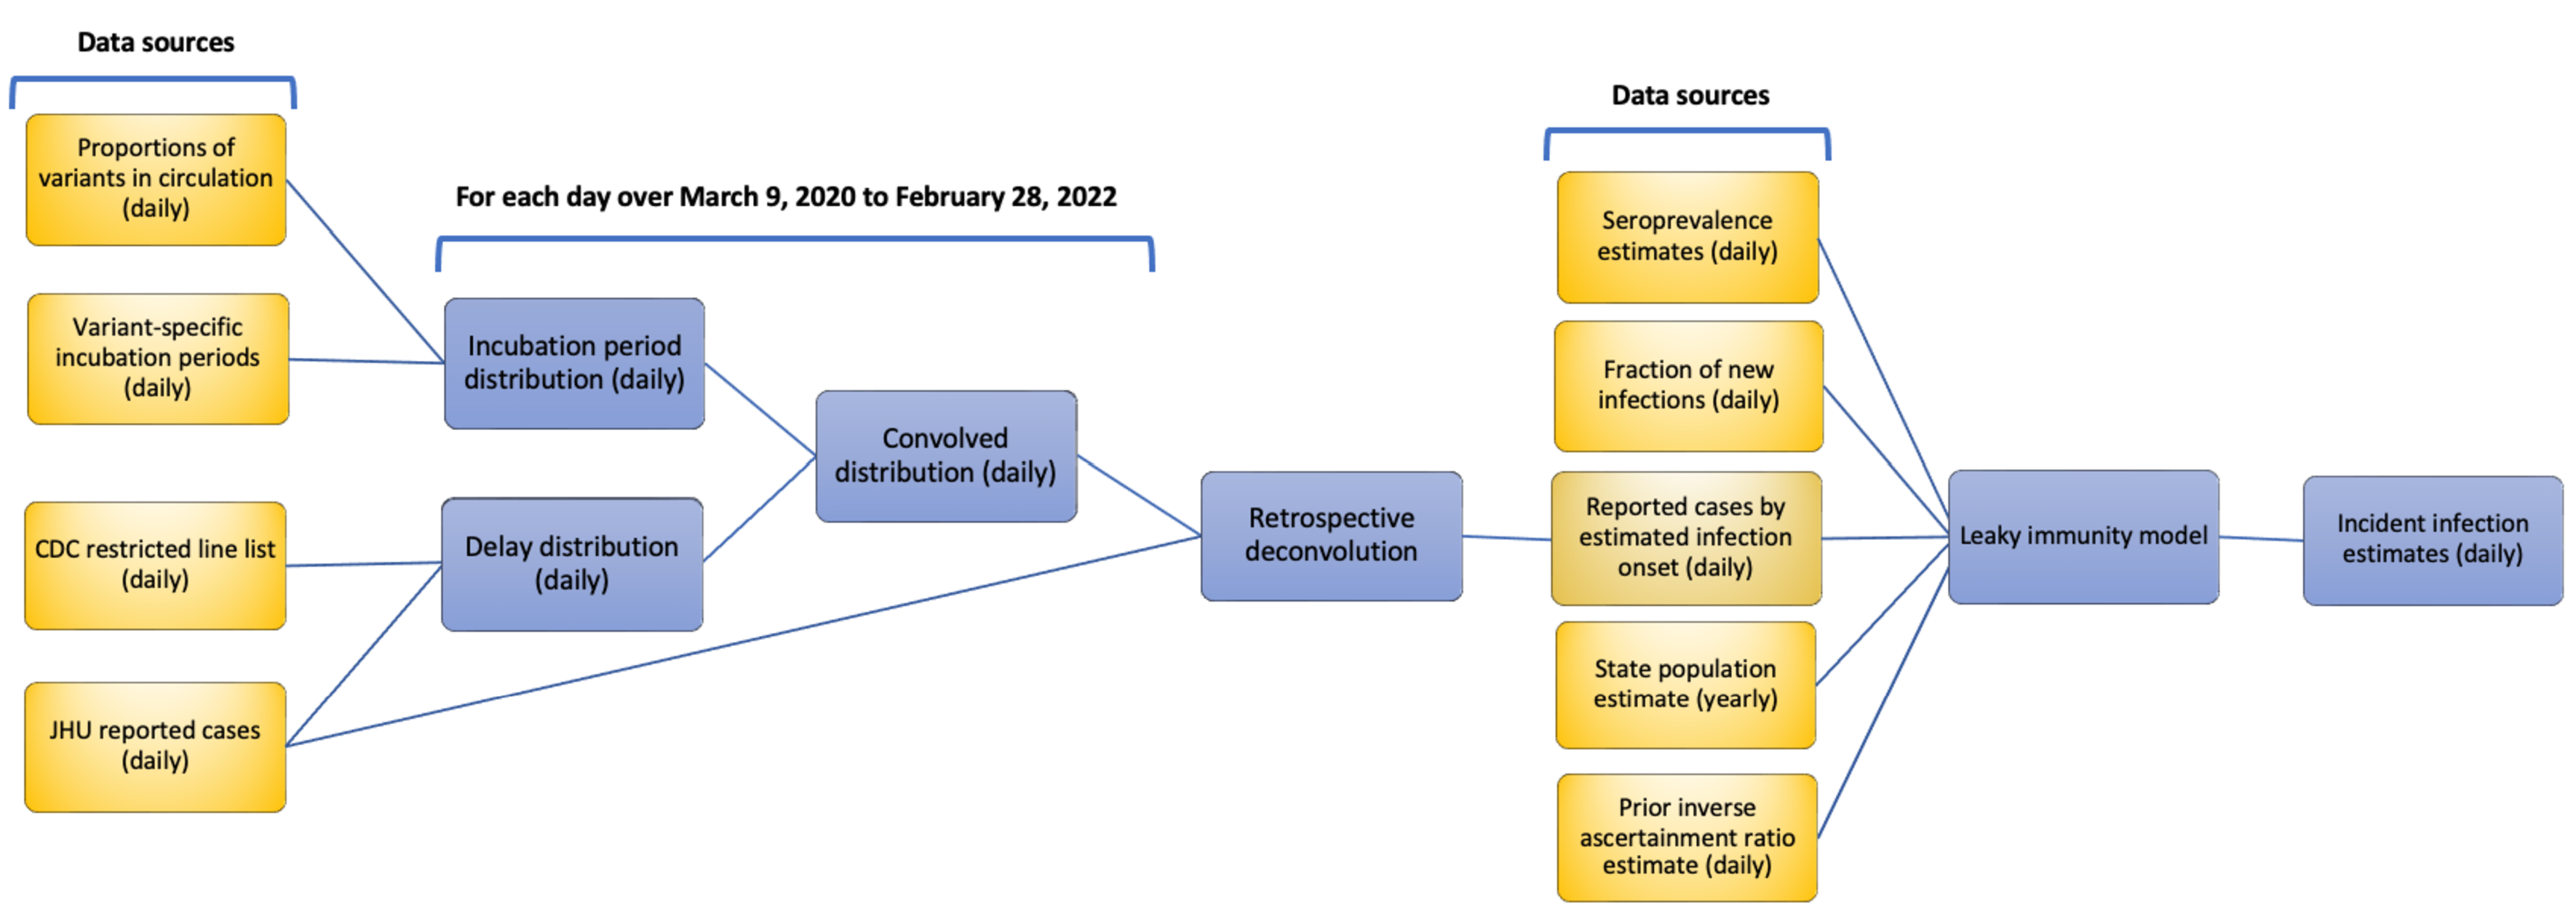
\includegraphics[width=.99\textwidth]{Reported_cases_to_infect_flowchart.pdf} 
    \caption{Flowchart of the inputted data and major analysis steps required 
    to get from reported cases to incident infection estimates for each day 
    over June 1, 2020 to Dec. 5, 2021 for a state. Data sources are coloured 
    in yellow, while data analysis steps are coloured in blue.}
    \label{fig:cases_to_infect_flowchart}
\end{figure}


\subsection{Data} 


The variant-specific incubation periods are taken to be the same for all states.
They are built using literature estimates of the gamma distribution parameters
or, if those are not readily available, the mean and standard deviation of the
number of days of incubation. Since the literature is lacking on reliable
estimates for the incubation period of Epsilon and Iota, we decided to use the
incubation period for Beta for both because Epsilon, Iota, and Beta are all
children from the same parent in the phylogenetic tree of the Nextstrain Clades
(as depicted in \citet{hodcroft2021covariants}).

To estimate the daily proportions of the variants circulating in each state, we
obtain the GISAID genomic sequencing data counts from CoVariants.org
\citep{hodcroft2021covariants, elbe2017data}\footnote{The complete list of
EPI\_SET Identifiers that were used to produce the CoVariants data are provided
in the Acknowledgements section of their website
\citep{hodcroft2021covariants}}. Since these counts are biweekly totals, we use
a simple convex optimization approach to interpolate daily numbers, where we
enforce that the counts in each interval must sum to the right boundary (the
biweekly total) and linear growth between the pairs of adjacent days. 

The COVIDcast API \citep{reinhart2021open} is used to retrieve the daily number
of new confirmed COVID-19 cases for each state that are based on reports from
the John Hopkins Center for Systems Science and Engineering (JHU CSSE)
\citep{dong2020interactive}. From the same API, we also retrieve the daily
number of confirmed COVID-19 hospital admissions for each state that are
collected by the U.S. Department of Health and Human Services (HHS). Both
datasets are as of June 6, 2022.

We obtain de-identified patient-level line list data on COVID-19 cases from the
CDC. Although there are both public and restricted versions of the dataset
available containing the same patient records \citep{cdc2020casepub,
cdc2020caserestr}, the restricted dataset\footnote{The CDC does not take
responsibility for the scientific validity or accuracy of methodology, results,
statistical analyses, or conclusions presented.} is selected because it contains
information on the state of residence which is essential for constructing
state-specific delay distributions. Since the restricted dataset is updated
monthly and cases may undergo revision, we use a single version of it that was
released on June 6, 2022. We consider this version to be finalized in that it
well-beyond our study end date such that the dataset is unlikely to be subject
to significant revisions.

In this dataset, the two key variables of interest are the dates of symptom
onset and report to the CDC. However, we find that the line list is prone to
high percentages of missing data, notably with respect to our variables of
interest. Nearly $60\%$ of cases are missing the symptom onset date, while about
$9\%$ of cases are missing the report date. In addition, we faced the
fundamental issue that \citet{jahja2022real} described, in which cases with
missing report dates may be filled with their symptom onset date.
\autoref{fig:prop_cc_zero_delay} suggests that this impacts states
to varying degrees due to the inconstant proportions of complete cases (those with
both onset and report date) that have zero delay between onset and report across
states. Due to this contamination in the zero delay cases (the true extent of
which is unknown to us), we omit all such cases from our analysis.

\begin{figure}[!tb]
\centering
    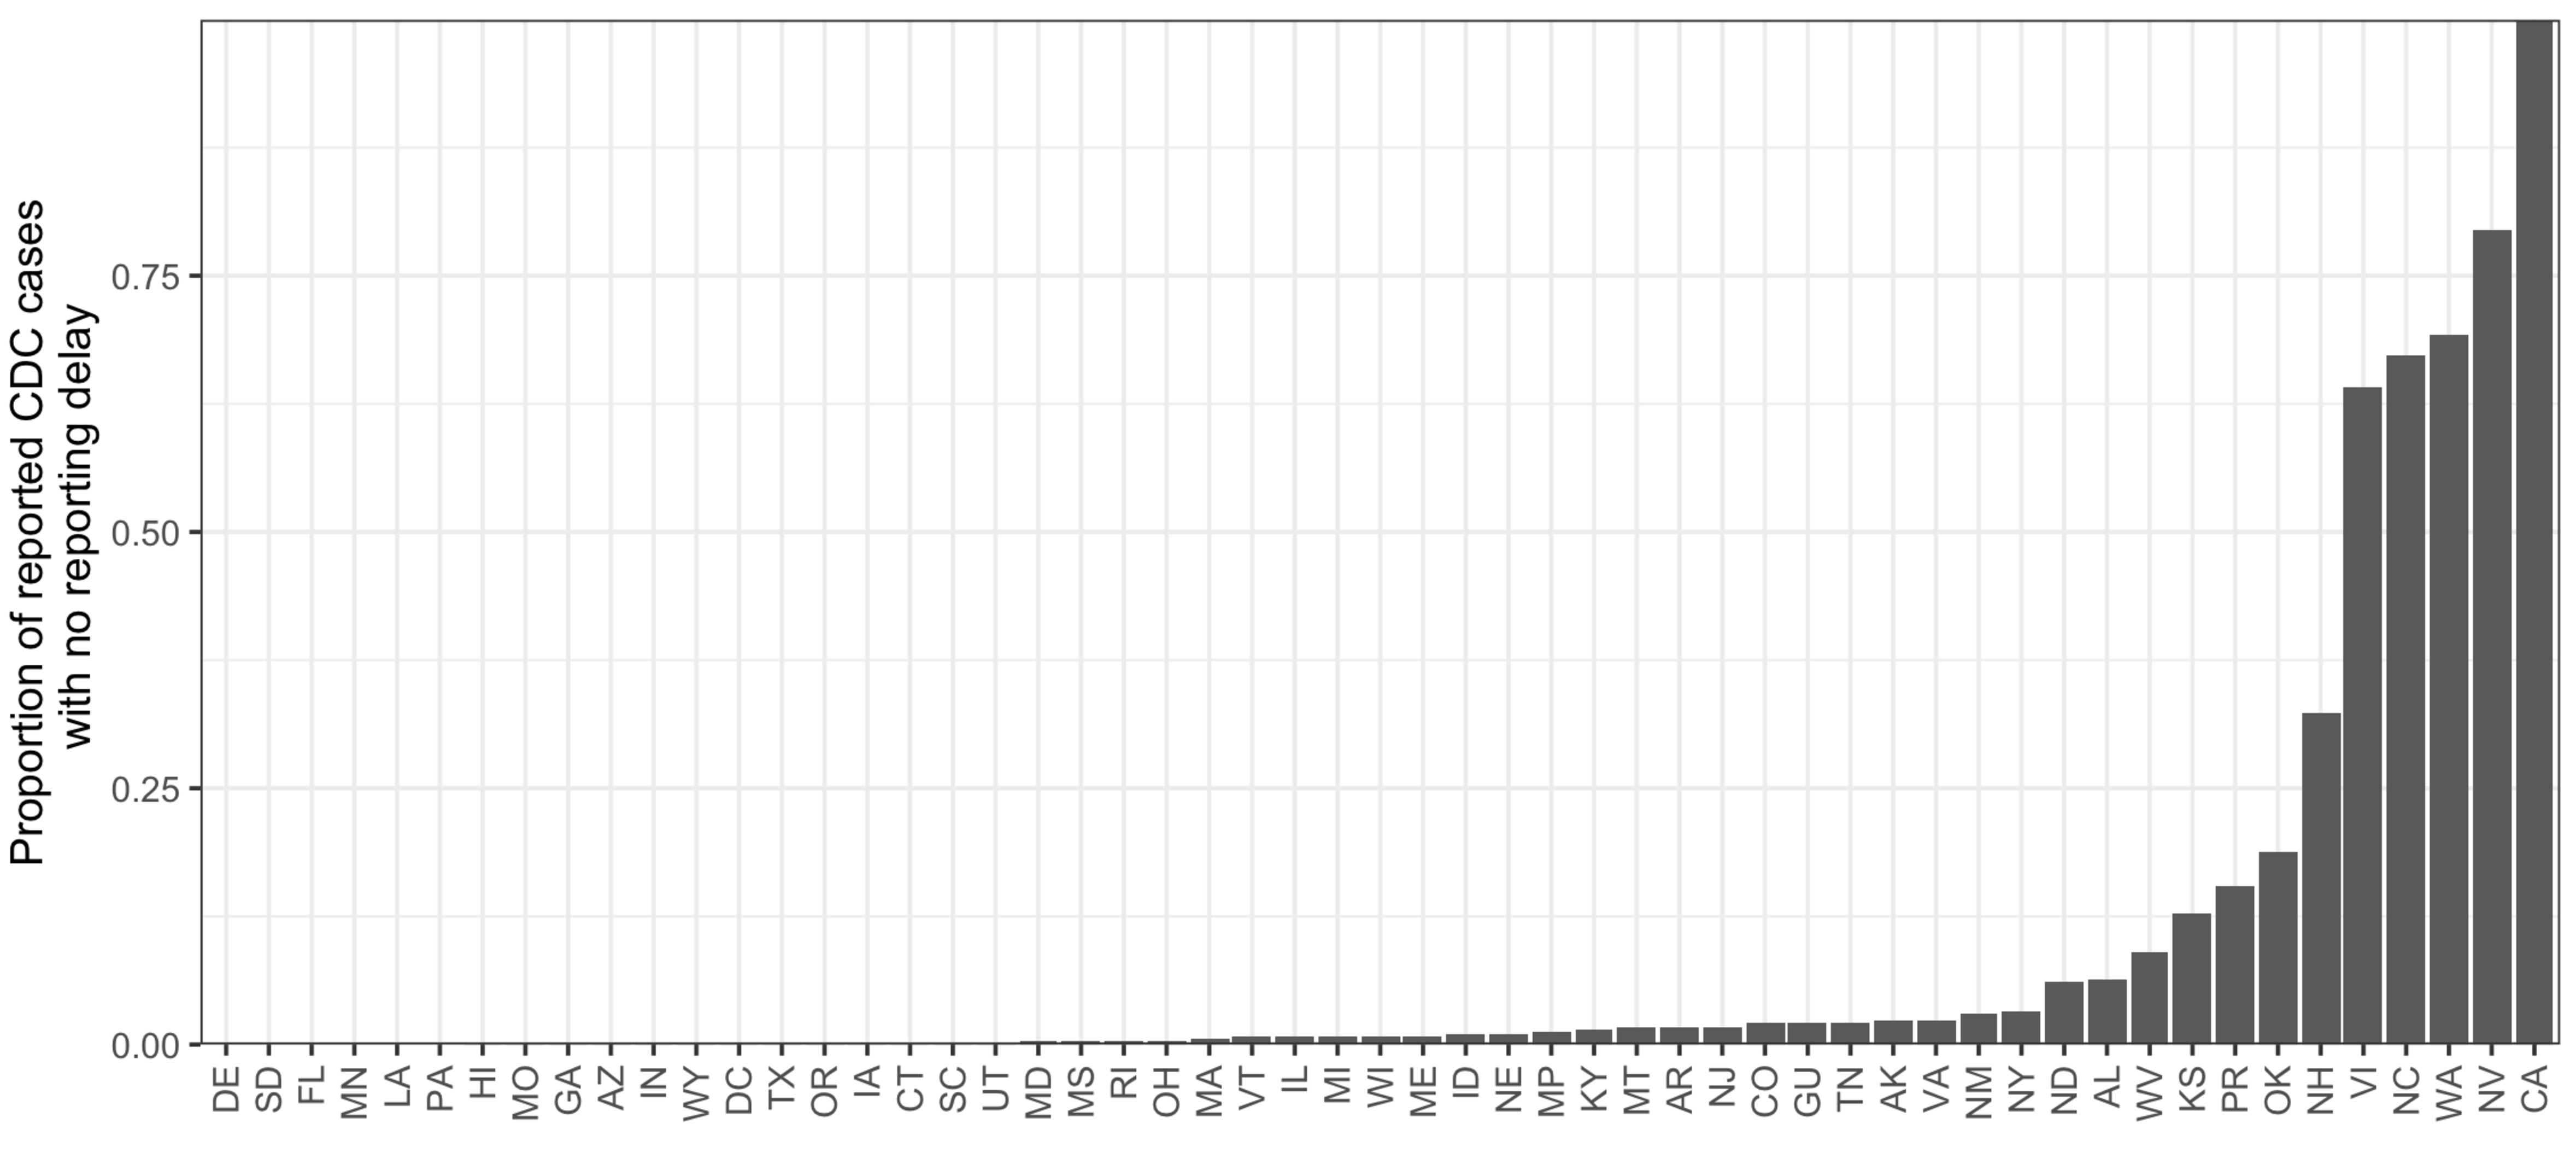
\includegraphics[width=.99\textwidth]{prop_cc_zero_delay.pdf}
    \caption{Proportion of complete cases with zero delay by state in the 
    restricted CDC line list dataset.}
    \label{fig:prop_cc_zero_delay}
\end{figure}

For the same release date, the restricted line list contains 74,849,225 cases
(rows) in total compared to 84,714,805 cases reported by the JHU CSSE; that is,
line list is missing about $10$ million cases for the same release date. The
extent that this issue impacts each state is shown in
\autoref{fig:prop_cc_cdc_vs_jhu}, from which it is clear the fraction of missing
cases is substantial for many states as it often surpasses $50\%$
\citep{jahja2022real}. In addition, the probability of being missing does not
appear to be the same for states, so there is likely bias introduced from using
the complete case line list data. We consider such bias to be unavoidable in our
analysis due to a lack of alternative line list sources.

\begin{figure}[!tb]
\centering
    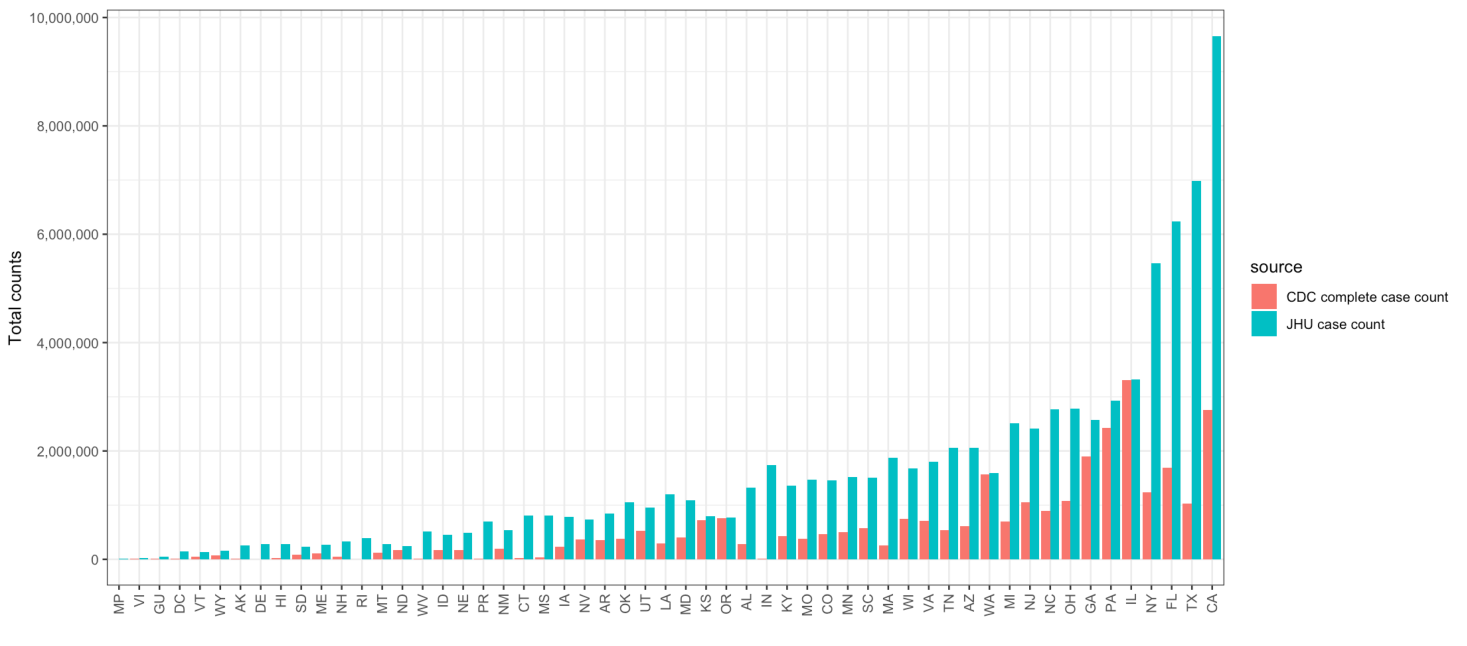
\includegraphics[width=0.99\textwidth]{prop_cc_cdc_vs_jhu.pdf} 
    \caption{Complete case counts by state in the CDC line list versus the 
    cumulative complete case counts from JHU CSSE as of June 6, 2022.}
    \label{fig:prop_cc_cdc_vs_jhu}
\end{figure}

In the line list, we observe unusual spikes in reporting in 2020 in comparison
to 2021. When plotting by report date, we find that a few states are
contributing unusually large case counts on isolated days very late in the
reporting process (usually well beyond $50$ days). We strongly suspect that
these large accumulations of cases over time are due breakdowns of the reporting
pipeline (which may be expected to occur more frequently in the year following
its instantiation than later on). Such anomalies are not likely to be reliable
indicators of the delay from symptom onset to case report. Therefore, we devise
a simple, ad hoc approach to detect and prune these reporting backlogs. 

For each of three considered dates, June 1, 2020, September 1, 2020, and
December 1, 2020 (which are chosen so that we do not include a case more often
than is necessary in the pruning process), we bin the reporting delays occurring
from $50$ days up to the maximum observed delay. Then, for each bin, we obtain
the total delay count for each state. We then check whether each count on the
log scale is at least the median (for the bin) plus $1.5$ times the
interquartile range and retain only those that met this criterion as potential
candidates for pruning. Next, we compute the counts by report date for each
candidate state. If there is a report date with a count greater than or equal to
the pre-specified threshold, then we remove those cases from the line list.
Based on inspection and intuition, we set the threshold to be $2000$ for the
first two bins, and then $500$ for all remaining bins. A similar trial and error
approach is used to set the bin size (to $50$ days). % Area for sensitivity
% analysis? Also, could discuss the choice of using only 3 dates 

To estimate the proportion of the population in each state with evidence of
previous infection across time, we use two major seroprevalence surveys that
were led by the CDC: the 2020-2021 Blood Donor Seroprevalence Survey and the
Nationwide Commercial Lab Seroprevalence Survey \citep{cdc2021blood,
cdc2021comm}. In the former, the CDC collaborated with $17$ blood collection
organizations in the largest nationwide COVID-19 seroprevalence survey to date
\citep{cdc2021blood}. The blood donation samples were used to construct monthly
seroprevalence estimates for nearly all states from July 2020 to December 2021
\citep{jones2021estimated}. In the latter survey, the CDC collaborated with two
private commercial laboratories and used blood samples to test for the
antibodies to the virus from people that were in for routine or clinical
management (presumably unrelated to COVID-19) \citep{bajema2021estimated}. The
resulting dataset contains seroprevalence estimates for a number of multi-week
collection periods starting in July 2020 to February 2022. 

Both datasets are based on repeated, cross-sectional studies that aimed, at
least in part, to estimate the percentage of people who were previously infected
with COVID-19 using the percentage of people from a convenience sample who had
antibodies against the virus \citep{bajema2021estimated, cdc2020data,
jones2021estimated}. Adjustments were made in both for age and sex to account
for the demographic differences between the sampled and the target populations.
However, both datasets are incomplete and they differed in the number and the
timing of the data points for each state (\autoref{fig:sero_blood_comm_compar}).
For example, in the commercial dataset, the last estimate for North Dakota is in
September 2020. In the blood donor dataset, Arkansas does not have estimates
available until October 2020. Furthermore, this blood donor dataset lacks
measurements for any states in 2022 (as the corresponding survey ended in
December 2021). Due to these limitations, reliance upon only one seroprevalence
survey is ill-advised for our purposes. 

\begin{figure}[!tb]
\centering
    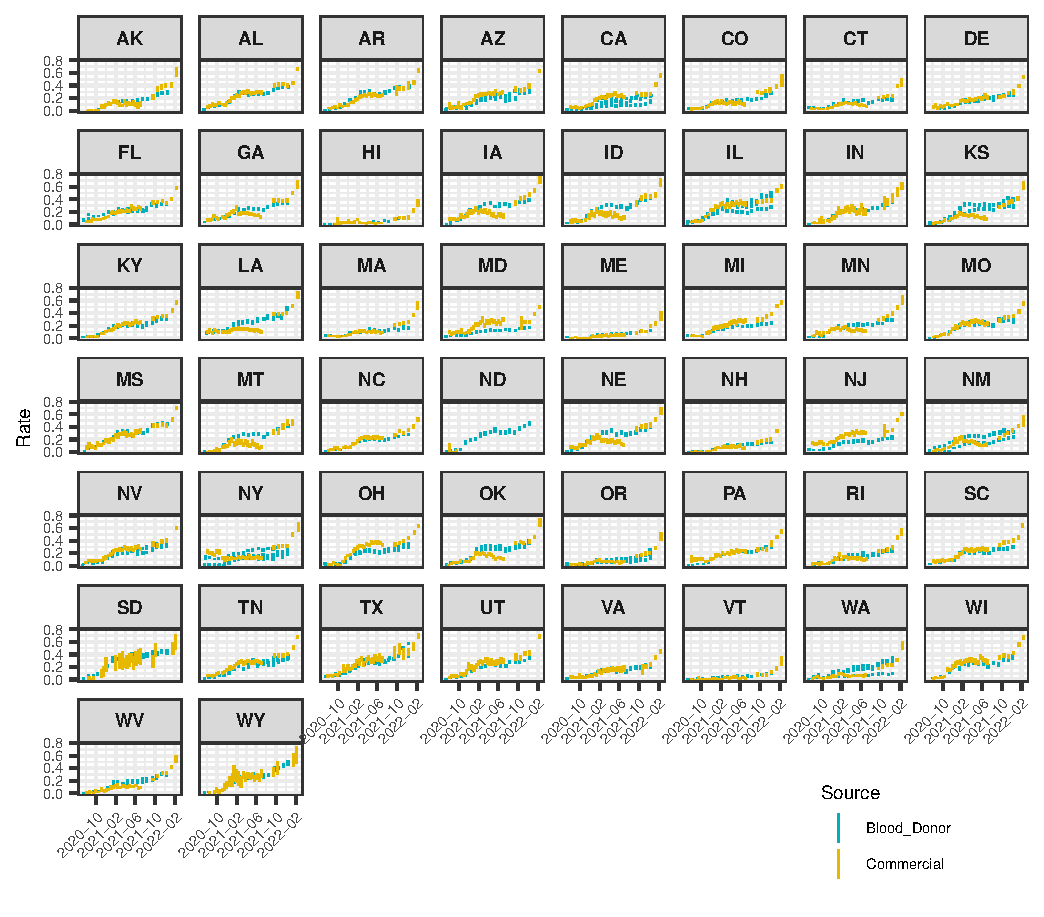
\includegraphics[width=.99\textwidth]{sero_blood_comm_compar.pdf}
    \caption{A comparison of the seroprevalence estimates from the Commercial
    Lab Seroprevalence Survey dataset (yellow) and the 2020-2021 Blood Donor 
    Seroprevalence Survey dataset (blue). Note that the maximum and the minimum
    of the line ranges are the provided 95\% confidence interval bounds to 
    give a rough indication of uncertainty.}
    \label{fig:sero_blood_comm_compar}
\end{figure}

The date variables that came with the two seroprevalence datasets were not the
same and so the date variables that we are able to construct from them are
different. For the commercial dataset, we use the midpoint of the provided
specimen collection date variable. A major difference in the structure of the
two datasets is that the commercial dataset always has the seroprevalence
estimates at the level of the state, while the blood donor dataset can either have 
estimates for the state or for multiple separate regions within the state. So for the 
blood donor dataset, we use the median donation date if the seroprevalence 
estimates are designated to be for entire state. If they are instead for regions in 
the state, since there is reliably one measurement per region per month, we 
aggregate the measurements into one per month per state by using a weighted 
average (to account for the given sample sizes of the regions). The median of the 
median dates is taken to be the date for the weighted average.

For adjusting our infection counts, annual estimates of the resident state
populations as of July 1 of 2020, 2021, and 2022 are taken from the December
2022 press release on the US Census Bureau website \citep{uscensus2022annual}.

The daily fraction of new infections are estimated from the provided incidence
of suspected reinfections over March 2020 to April 2022 in Clark County, which
is based on surveillance work conducted by the Southern Nevada Health District
(SNHD) and reported by \citet{ruff2022rapid}. The proportion of new cases per
week that are suspected reinfections are calculated by dividing the number of
suspected reinfections by all new PCR-identified cases during the same week. 
%Possible problem here – reinfections not include third infections (see comments
% in the discussion section about this)

\subsection{Incubation period distribution estimation} 

For each state at each time over June 1, 2020 to December 5, 2021, we estimate
the incubation period distribution from a finite and countable mixture of gamma
distributions to account for the gradual decline in the incubation period across
variants. The variants considered are Alpha, Beta, Gamma, Delta and Omicron,
which are designated as variants of concern by WHO based on their potential to
cause new waves, dethrone the dominant variant, and lead to changes in public
health policy \citep{who2021tracking}. In addition, we include the Epsilon
(California) and Iota (New York) variants because of their impact on those and
the surrounding states \citep{yang2022investigation, duerr2021dominance}. We
relegate all other variants to be in an Other category (so that the proportions
circulating in a state at a time always sum to one). This decision is, in part,
motivated by the lack of sequencing data for most states in 2020 as well as the
presence of an others category in the sequencing data for that time. 
% Perhaps include heatmap(s) from https://docs.google.com/document/d/1WSa_CN5gXsa-5Ozuj6xZt2-knflL507QdwiiRscaW2o/edit
Then, for each variant in a state at a time, the proportion of the variant
circulating (the mixture weight) is multiplied by the corresponding component
gamma distribution for the incubation period. These distributions are the same
for all states and based on literature estimates of the gamma parameters or the
mean and standard deviation of the incubation period (in which case the method
of moments is used to fit a gamma density). Finally, we discretized the
resulting mixture density to the support set, which is taken to be from $1$ and
$21$ days. In other words, those are taken to be the lower and upper limits for
the number of days that the virus could be incubating in someone. The implicit
assumption for the lower bound is that there must be at least one day between
infection and symptom onset (which follows the convention given in
\citet{phcan2021covid}). The assumption underlying the upper bound is that $21$
days is the maximum number of days that the virus could be incubating in someone
(which is reasonable based on \citet{zaki2021estimations} and
\citet{cortes2022sars}).

\subsection{Delay distribution estimation} 

We use the restricted CDC line list to estimate the distribution between symptom
onset and report for each state at each time. For brevity and consistency with
\citet{jahja2022real}, let this be known as the delay distribution. More
formally, let $y_t$ denote the count of new cases reported at time $t$ and $x_t$
denote the count of new infections with onset at $t$ for a state. Solely from
knowing that each case had both an onset and a report date (ie. is a complete
case), we can count the cases that are reported at time $t$ by enumerating
them according to onset (as in \citet{jahja2022real}):
\begin{align*}
y_t = \sum_{s=1}^{t} \sum_{i=1}^{x_s}1 \left ( \text{the }i\text{th infection at }
 s \text{ gets reported at }t \right )
\end{align*}
Taking the conditional expectation of the above yields
\begin{align*}
E(y_t | x_s, s \leq t) = \sum_{s=1}^{t} \pi_t(s) x_s 
\end{align*}
where $\pi_t(s) = P(\text{case report at }t| \text{infection onset at }s)$ for
each $s \leq t$ are the delay probabilities and the $\left( \pi_t(s) : s \leq t
\right)$ sequence comprises the delay distribution at time $t$. Notice that
there are no time restrictions placed on the infection onset save that it must
have been between the first time and the report date, inclusive. This is
unlikely to be a realistic assumption to make as $t$ moves farther away from
$s$. 

Thus, we make two key assumptions about the delay distributions. Firstly,
infections that are reported to the CDC are always reported within $d = 60$
days, which is chosen because the vast majority of cases are found to be
reported within $60$ days. Secondly, the probability of zero delay is zero,
which stems from the contamination of zero delay in the line list. 

As in \citet{jahja2022real}, we update the conditional expectation formula to
reflect these two assumptions: 
\begin{align*}
E(y_t | x_s, s \leq t) = \sum_{k=1}^{d} p_t(k) x_{t-k}
\end{align*}
where for $k = 1, \dots, d$,
\begin{align*}
p_t(k) = P(\text{case report at }t | \text{infection onset at }t-k).
\end{align*}

For each state, we estimate the delay distribution (ie. the probabilities for
$1$ to $60$ days of delay) at each $t$ by using the empirical distribution of
all non-zero lags between the complete cases whose onset dates fall in the
center-aligned interval about $t$ designated by $\left[ t - 1.25d + 1, t + d
\right]$). 

Now, the task of estimating the delay distribution for each state at each time
can be described by four distinct steps. First, we obtain the empirical
distribution of all lags (excluding zero) from all cases with onset dates
falling in the center-aligned interval. Next, we weight the state-specific
empirical distribution by the proportion of CDC to JHU cases. That is, we
compare the number of CDC cases used to make the empirical distribution to the
number of JHU reported cases in the time window of $\left[t - d + 2, t +
1.25d\right]$ (to correspond appropriately to the center aligned interval for
the CDC cases). This proportion is used as the weight for the state’s empirical
distribution, while the complement is used to weight the overall empirical
distribution that is forged from the data for all states. This construction
allows for more reliance on the state's distribution when there are more CDC
cases relative to JHU (and vice versa). After implementing the shrinkage method,
we fit a gamma density to the resulting empirical distribution by the method of
moments. Finally, we discretize the resulting density to the support set of $1$
to $d = 60$ days.
 
\subsection{Convolution} 

From the incubation period and delay distribution estimation, we acquire one
delay and one incubation period distribution for each state at each time under
consideration. We then convolve each pair of distributions to get the estimated
infection-to-report distributions and, hence, the estimated probabilities for
the delay from infection onset to case report. 

\subsection{Retrospective deconvolution}

The goal for retrospective deconvolution is to estimate the daily number of new
infections in the above conditional expectation formula. For each state, we
achieve this goal by solving the following optimization problem. 

Following the notation of \citet{jahja2022real} (save for suppressing the
state/location subscript), let $T$ represent the deconvolution period from June
1, 2020 to December 5, 2021. Let $\hat{p}_t$ be probabilities from the estimated
infection-to-report distribution for $t \in T$, $y_t$ the number of new cases
reported, and $D^{(4)}x$ yields all $4$th-order differences of the $x$ vector
(by using the discrete derivative matrix of order $4$, $D^{(4)}$). From these,
we estimate the latent infection counts for the reported cases across time by
solving for the vector $x$ in
\begin{align*}
\min_{x} \sum_{t \in T} \left ( y_t -  \sum_{k = 1}^{d} \hat{p}_t(k)x_{t-k} 
\right )^2 + \lambda \|D^{(4)}x\|_1. 
\end{align*}

The above loss function decouples into two parts with competing interests (that
encapsulate the classic bias-variance trade off). The first part represents
minimising the sum of squared residuals between the JHU reported cases and the
fitted values, while the second part captures the smoothness (between every set
of five infection counts). The underlying idea here is to introduce bias to
reduce the amount of variance, so that the model is not overfit to the training
data.

We solve this trend-filtering-regularized least squares deconvolution problem by
employing the ADMM algorithm from \citet{ramdas2016fast} that is described in
Appendix A of \citet{jahja2022real}. The solution to the problem is an adaptive
piecewise cubic polynomial estimate \citep{tibshirani2014adaptive,
tibshirani2022divided}.

We select the tuning parameter, $\lambda$, by using $3$-fold cross validation as
in \citet{jahja2022real} in which every third incident infection count is
reserved for testing and imputed with the average of the two surrounding counts.
We use each imputed count to construct a fitted value and compare it to the
actual number of new cases reported. The tuning parameter that resulted in the
smallest sum of squared residuals is ultimately chosen.

\subsection{Inverse reporting ratio and the leaky immunity model} 

The infection estimates from retrospective deconvolution are
derived solely from the infection onset dates of the reported cases. Hence,
to capture the unreported infections, it is necessary to adjust those estimates by 
a scaling factor that approximates the ratio of the true number of new infections
to the new reported infections. We refer to this quantity as the
inverse reporting ratio and denote it by $a_t$ for time $t$. Our new goal is
to estimate this quantity for every state at every time under consideration. 

Now, we already acquired the new number of reported infections from our
unadjusted estimates (produced by deconvolution). As for the new true
infections, since seroprevalence of anti-nucleocapsid antibodies is used to
estimate the percentage of people who have at least one resolving or past
infection \citep{cdc2020data}, we can use the change in subsequent
seroprevalence measurements to estimate this quantity. Hence, we adjust the 
retrospective deconvolution estimates using a model that is based on the 
seroprevalence. With the subscript for the state suppressed (to avoid 
cluttering the notation), let $s_t$ be a seroprevalence estimate at time $t$, $w_t$ be
 the inverse variance weights derived from those
estimates, and $\Delta R_t$ be the change in cumulative reported infections 
scaled by the state’s population. To account for reinfections, we multiply the 
change in reported infections at time $t$ by the corresponding fraction
 of new infections, $n_t$. Using these components, we construct the 
 following objective function separately for each state
\begin{align}
\min_{a, \gamma}\frac{1}{2}\sum_{t \in T}w_t\left (s_t - (1 -\gamma)s_{t-1} 
- a_t\Delta R_t n_t  \right )^2 + \frac{\lambda}{2} \|D^{(3)}a\|_2^2 \label{eq:leakypr}
\end{align}
where $D^{(3)}$ is the discrete derivative matrix of
order $3$, lambda is the tuning parameter, and $\gamma$ is the percentage of
 people who lose immunity between time $t$ and time $t+1$. 

We refer to $\gamma$ as the leaky parameter and we call this model leaky 
immunity model. By ``leaky'' we mean the decrease in detectability of antibodies 
due to the natural degradation of infection-induced
immunity over time. Since the true course of immunity over time is unknown
\citep{goldberg2022protection}, we take this rather straightforward approach 
and simply model a singular $\gamma$ to try
avoid making gratuitous or overly restrictive assumptions.

\subsection{State space representation of the leaky immunity model}

To estimate the leaky immunity model in \autoref{eq:leakypr}, we express it as a 
Gaussian state space model (as in \citet{durbin2012time} and \citet{helske2017kfas}).

In general, for $t = 1, \dots, n$, we let $\alpha_t$ be the $m \times 1$ vector of latent
state processes at time $t$ and $y_t$ be the $p \times 1$ vector of observations
at time $t$. Under the assumption that $\eta$ is a $k \times 1$ vector, the
form of the linear Gaussian state space model is 
\begin{align}
y_t &= Z_T\alpha_t + \epsilon_t  \text{     (observation equation)} \label{eq:ss1}\\
\alpha_{t+1} &= T_t\alpha_t + R_t\eta_t  \text{     (state equation) \label{eq:ss2}}
\end{align}
where $\epsilon \sim N(0, H_t)$, $\eta \sim N(0, Q_t)$, and $\alpha_1 \sim
N(a_1, P_1)$ independently of each other \citep{helske2017kfas}. For notational
compactness, we let $\alpha = \left ( \alpha_1^T, \dots, \alpha_n^T \right )$
and $y = \left ( y_1^T, \dots, y_n^T \right )$.

The observation equation can be viewed as a linear regression model with the
time-varying coefficient $\alpha_t$, while the second equation is a first-order
autoregressive model, which is Markovian in nature \citep{durbin2012time}. 

The main idea of the two equations is that the system evolves over time
according to $\alpha_t$ (as in the second equation), but since those states are
not directly observed, we turn to the observations $y_t$ and use their
relationship with $\alpha_t$ (as in the first equation) to drive the system
forward \citep{durbin2012time}. So the objective of state space modeling is to
obtain the latent states $\alpha$ based on the observations $y$ and this is
achieved through Kalman filtering and smoothing. 

Kalman filtering gives the one-step-ahead predictions and prediction errors:
\begin{align*}
a_{t+1} &= \textup{E}(\alpha_{t+1}|y_t, \dots, y_1) \\
v_t &= y_t - Z_ta_t
\end{align*} with covariance, 
\begin{align*}
P_{t+1} &= Var(\alpha_{t+1}|y_t, \dots, y_1) \\
Var(v_t) &= Z_tP_tZ_t^T + H_t.
\end{align*}
Then, the state smoothing equations are run back in time to give
\begin{align}
\hat{a}_t &= E(\alpha_{t}|y_n, \dots, y_1) \label{eq:hatat}\\
V_t &= Var(\alpha_{t}|y_n, \dots, y_1). \label{eq:Vt}
\end{align}
The filtering and smoothing steps are based on recursions that are described in
Appendix A of \citet{helske2017kfas} as we use the R package KFAS to estimate
our model.

% Maybe include the following somewhere, though perhaps not necessary:
% We should note that the Kalman filter and smoothing approach offers a number of
% advantages over the penalized regression approach for our situation. For
% example, the parameters are estimated all at once (so cross validating for model
% parameter tuning is not necessary). In addition, it can handle unevenly spaced
% time series and and forward/backward extrapolation can be used to extrapolate
% outside the observed seroprevalence range (refer to \citet{durbin2012time} for
% further details).

The leaky immunity model can be written in state space form by defining the
components in Equations \ref{eq:ss1} and \ref{eq:ss2} as follows:

% Probably move the below specification to the appendix

\begin{alignat*}{3}
R &= \begin{bmatrix}
1 & 0 & 0 \\ 
0 & 1 & 0\\ 
0 & 0 & 1\\ 
0 & 0 & 0\\ 
0 & 0 & 0 
\end{bmatrix} &\qquad 
Z &= \begin{bmatrix}
1 & 0 & 0 & 0 & 0 \\ 
0 & 1 & 0 & 0 & 0
\end{bmatrix} &\qquad 
H &= \begin{bmatrix}
0 & 0 \\ 
0 & 0
\end{bmatrix} \\
\alpha_t &= \begin{bmatrix}
s_{t,c}\\
s_{t,b}\\ 
a_t\\ 
a_{t-1}\\ 
a_{t-2}
\end{bmatrix} & 
T_t &= \begin{bmatrix}
 \gamma & 0 & \Delta R_tn_t & 0 & 0\\ 
 0 & \gamma & \Delta R_tn_t & 0 & 0 \\ 
 0 & 0 & 3 & -3 & 1 \\ 
 0 & 0 & 1 & 0 & 0\\ 
 0 & 0 & 0 & 1 & 0
\end{bmatrix}  & 
Q_t &= \begin{bmatrix}
w_{t,c}\sigma^2_s & 0 & 0 \\ 
0 & w_{t,b}\sigma^2_s  & 0 \\ 
0 & 0 & \sigma^2_a
\end{bmatrix} \\
a_1 &= \begin{bmatrix}
\tilde{s}_{1,c}\\ 
\tilde{s}_{1,b}\\ 
\tilde{a}_1\\ 
\tilde{a}_1 \\
\tilde{a}_1
\end{bmatrix} & 
P_{1} &= \begin{bmatrix}
\sigma^2_{\tilde{s}_{1,c}} & 0 & 0 & 0 & 0\\ 
0 & \sigma^2_{\tilde{s}_{1,b}} & 0 & 0 & 0\\ 
0 & 0 & \sigma^2_{\tilde{a}_1} & 0 & 0\\ 
0 & 0 & 0 & \sigma^2_{\tilde{a}_1} & 0 \\ 
0 & 0 & 0 & 0 & \sigma^2_{\tilde{a}_1}
\end{bmatrix} 
\end{alignat*}
where $\sigma^2_s$ is the variance of observations (common across time) and
$\sigma^2_a$ is the trend variance. Letting the subscripts $b$ and $c$ denote
the blood donor and commercial datasets, $w_{t,c}$ and $w_{t,b}$ are the
time-varying inverse variance weights computed from the commercial and blood
donor datasets, respectively. 

For each source, we compute the weights for the observed seroprevalence
estimates using the standard formula for the standard error of a proportion.
These weights are then re-scaled so they sum to the number of observed
seroprevalence measurements for the source. All days that are unobserved (ie.
lack seroprevalence measurements) are given weights of one. Finally, the ratio
of the average observed weights for the sources is used as a multiplier to scale
all of the weights for one source. For example, if the average weight of the
commercial source is double the average weight of the blood donor source (for an
arbitrary state), then we scale all of the weights in the commercial source
(including the ones) by two. The main purpose of this step is to to ensure that
the source with a greater sample size contributes more weight in the model on
average. % Is the red sentence quite right or is it just that the source with larger
%weights on average will have more weight? 

The prior distribution for $\alpha_1$ is estimated using both data-driven constraints 
and externally sourced information. The initial values of the two seroprevalence 
components are expected to be close to
but smaller than the first observed value from the sources. Hence, we
extract the first observed seroprevalence measurement from each source, round
those down to two decimal places, and take those to be the estimated initial
values $\tilde{s}_{1,c}$ and $\tilde{s}_{1,b}$. The corresponding initial
variance estimates of $\sigma^2_{\tilde{s}_{1,c}}$ and
$\sigma^2_{\tilde{s}_{1,b}}$ are obtained from the formula for the standard
error of a proportion. For all of the initial values of the trend components, 
 we use the inverse of the ascertainment ratio estimate as of June 1, 2020 for each state
from Table 1 in \citet{unwin2020state} and denote this by $\tilde{a}_1$. The
initial variance estimate of $\sigma^2_{\tilde{a}_1}$ is based on the variance implied 
by the given inverse ascertainment ratio distribution.
% standard deviation implied by the interval in that table.  
% Update this last sentence if end up going with the standard deviation implied by the interval in Table 1
% instead of the variance implied by u_m ~ Beta(12,5) from the unwin2020state paper

The initial $\sigma^2_s$ is taken to be the average of the estimated variances
from the linear models for the sources where the observed seroprevalence
measurements are regressed on the enumerated dates. The initial value of
$\lambda$ is taken to be $100$ and is based on inspection.  

Following the maximum likelihood estimation of the unknown parameters, $\gamma$,
$\lambda$, and $\sigma^2_s$, we use the Kalman filtering and smoothing to obtain the
smoothed estimates of the states (which are the inverse reporting ratios) and
their covariance matrices as shown in Equations \ref{eq:hatat} and \ref{eq:Vt}.
Forwards and backwards extrapolation is used to estimate the ratios outside of the 
observed seroprevalence range \citet{durbin2012time}. After we obtain one vector of 
inverse reporting ratios for each state in this
way, we take each inverse reporting ratio and multiply it by the corresponding
unadjusted estimate to obtain an adjusted estimate of new infections for each
state at each time. We are able to convert these numbers of infections to
infections per $100,000$ population by simple re-scaling (enabled by the fact
that normality is preserved under linear transformations).

The $50$, $80$, and $90\%$ confidence intervals are constructed by taking a
Bayesian view of the leaky immunity model (refer to the Online
Supplement~\ref{supp:bayesleaky} for the Bayesian specification of the leaky
immunity model). That is, for each time, $t$, we obtain an estimate of the
posterior variance of $a_t$, apply the unadjusted estimate as a constant
multiplier, and then use resulting variance to build a normal confidence
interval about the adjusted estimate. We additionally enforce that the lower
bound must be at least the unadjusted estimate for the time under consideration.

\subsection{Lagged correlation to hospitalizations} 

We use our adjusted infection estimates in a lagged correlation analysis with
confirmed COVID-19 hospitalizations. Our primary goal of this analysis is to
find the lag between infection and hospitalization rates that gives the highest
average rank-based correlation across US states. To that end, we consider a wide
range of possible lag values ranging from $1$ to $50$ days. Zero and negative
lags are not considered because COVID-19 infection onset must precede
hospitalization due to the virus. To remove day of the week effects, both the
adjusted infections and hospitalization signals are subject to a $7$-day moving
average (center-aligned) before their conversion to rates.

For each state and over all days in the June 1, 2020 to December 5, 2021 time
period, we compute the (Spearman’s) correlation between and infection and
hospitalization rates for each lag using the epi\_cor function from the
epiprocess package \citep{brooks2023epiprocess}. We then calculate the average
correlation across all states for each lag. The lag that led to the highest
average correlation is then used to estimate the time-varying IHRs for each
state. To compute this for a given day, the number of individuals who are
hospitalized due to COVID-19 on a day are divided by the estimated total number
who were infected on the lagged number of days before.

%#%% Question for Ryan and Maria: In the Figure 3.16 caption from Maria’s
%thesis, she says that she computes The correlation is taken over a rolling
%window of d = 45 days. Should we be doing something similar (instead of
%computing the correlation For each state over all days)? Is that a lot more
%suitable than what we're currently doing?

\subsection*{Acknowledgements}

% Required Gisaid acknowledgement
We gratefully acknowledge all data contributors, i.e., the Authors and their
Originating laboratories responsible for obtaining the specimens, and their
Submitting laboratories for generating the genetic sequence and metadata and
sharing via the GISAID Initiative \citep{elbe2017data}, on which this research
is based.

%\bibliographystyle{naturemag} #%% Change back to numeric references in line with requirements for Nature Communications articles (see pg 3 fro here: https://www.nature.com/documents/ncomms-formatting-instructions.pdf)
\bibliographystyle{plainnat}

\newpage
\bibliography{bibliography.bib}

\newpage
% Eventually make the supplement a separate document with its own title page 
\beginsupplement
\title{Online Supplement} 
\maketitle
\section{Text}  
\subsection{Models}
\subsubsection{Bayesian specification of the leaky immunity
model}\label{supp:bayesleaky} In brief, the leaky immunity model where we let
$\beta = \left \{  \gamma, a_1,\dots, a_t \right \}$ and $X$ be the design
matrix, corresponds to a Bayesian model with prior 
\begin{align*}
    \beta \sim N \left( 0,  \frac{\sigma^2 }{ \lambda} \left( A^TD^TDA 
    \right)^{-1}  \right)
\end{align*} and likelihood 
\begin{align*}
    s|X,\beta \sim N \left( X\beta, \sigma^2W^{-1} \right),
\end{align*} where $A$ is indicator matrix save for the first column of $0$s 
(corresponding to $\gamma$), $D$ represents the discrete derivative matrix of 
order $3$, and $W$ is the inverse variance weights matrix. Then, the posterior 
on $a_t$ is normally distributed with mean 
\begin{align*}
    \left ( X^TWX + \lambda A^TD^TDA \right )^{-1}X^TWs
\end{align*} 
and variance 
\begin{align*}
    \sigma^2 (X^TWX + \lambda A^TD^TDA)^{-1}.
\end{align*}

\end{document}
